\documentclass[12pt]{article}
\usepackage{graphicx}
\usepackage{amsmath}
\usepackage{float}
\usepackage{hyperref}
\usepackage[margin=1in]{geometry}
\usepackage{bookmark}


\title{Optimizing E-Commerce Marketing Campaigns Using SEMMA: \\An Exploratory Data Analysis of the UCI Online Retail Dataset}
\author{Pruthvik Sheth\\
        San Jose State University\\
        \texttt{pruthvik.sheth@sjsu.edu}}
\date{}

\begin{document}

\maketitle

\begin{abstract}
Understanding customer behavior in e-commerce is crucial for crafting data-driven marketing strategies that maximize customer engagement and return on investment (ROI). This paper presents an exploratory data analysis (EDA) of the UCI Online Retail dataset using the SEMMA methodology—Sample, Explore, Modify, Model, Assess. We focus on identifying customer segments, predicting responses to different marketing campaigns, and providing actionable recommendations to optimize future campaign strategies. The analysis reveals key customer segments and highlights effective marketing channels based on customer engagement data.
\end{abstract}

\section{Introduction}
With the exponential growth of e-commerce, businesses are increasingly relying on data to optimize marketing strategies and drive customer engagement. Traditional marketing campaigns often lack the precision needed to engage customers effectively, leading to suboptimal returns on investment (ROI). This paper aims to explore customer behavior in an e-commerce context by analyzing the UCI Online Retail dataset \cite{uci_dataset}. Using the SEMMA (Sample, Explore, Modify, Model, Assess) methodology, we will uncover patterns in customer behavior, identify high-value customer segments, and provide data-driven recommendations for marketing campaign optimization.

\subsection{Objectives}
The key objectives of this analysis are:
\begin{enumerate}
    \item To identify customer segments based on purchasing behavior.
    \item To predict customer engagement with different marketing campaigns (e.g., email, social media, paid ads).
    \item To provide actionable recommendations for optimizing future marketing campaigns.
\end{enumerate}

\section{Methodology}
The SEMMA methodology guides the analysis process, dividing it into five key steps: Sample, Explore, Modify, Model, and Assess. This section describes how each step was implemented.

\subsection{Sample}
We begin by loading the UCI Online Retail dataset, which contains over 500,000 records of transactions between 2010 and 2011. To ensure computational efficiency, we sampled 10\% of the dataset after cleaning it for missing values and removing anomalies, such as negative or zero quantity transactions.

\subsection{Explore}
During the exploration phase, we conducted descriptive statistics and visualizations to uncover patterns in the data:
\begin{itemize}
    \item \textbf{Sales Over Time:} A time series analysis revealed monthly trends in total sales, with seasonal peaks observed during the holiday season.
    \item \textbf{Top Products:} The most frequently purchased products were identified, providing insight into customer preferences.
    \item \textbf{Customer Spending Distribution:} The distribution of customer spending was analyzed to identify high-value customers.
\end{itemize}

\subsection{Modify}
In the modification phase, several data preprocessing steps were conducted:
\begin{itemize}
    \item Negative and extreme quantities were handled by filtering out invalid transactions and capping extreme values at the 99th percentile.
    \item One-hot encoding was applied to categorical variables such as `Country` to prepare them for the modeling phase.
    \item Recency, Frequency, Monetary (RFM) analysis was used to segment customers based on their purchase behavior.
\end{itemize}

\subsection{Model}
For the modeling phase, we applied two main techniques:
\begin{itemize}
    \item \textbf{Clustering:} Using K-Means clustering, we identified three key customer segments: Loyal Customers, At-Risk Customers, and Potential Loyalists.
    \item \textbf{Predictive Modeling:} Logistic Regression and Random Forest models were used to predict customer responses to marketing campaigns. Feature importance from the Random Forest model provided insights into the most effective campaign channels.
\end{itemize}

\subsection{Assess}
The final assessment phase involved evaluating the models and providing recommendations:
\begin{itemize}
    \item The Logistic Regression model achieved higher performance compared to Random Forest, with an F1-score of 0.70.
    \item A silhouette score of 0.6 indicated well-defined customer clusters.
\end{itemize}

\section{Results}

\subsection{Customer Segmentation}
The K-Means clustering algorithm segmented customers into three distinct groups:
\begin{enumerate}
    \item \textbf{Loyal Customers:} These customers exhibit frequent purchases with high monetary value, and they made recent transactions.
    \item \textbf{At-Risk Customers:} This group consists of customers who have not made purchases recently and exhibit lower frequency and monetary value.
    \item \textbf{Potential Loyalists:} These customers show moderate engagement and have the potential to be converted into loyal customers with the right marketing strategies.
\end{enumerate}

\begin{figure}[H]
\centering
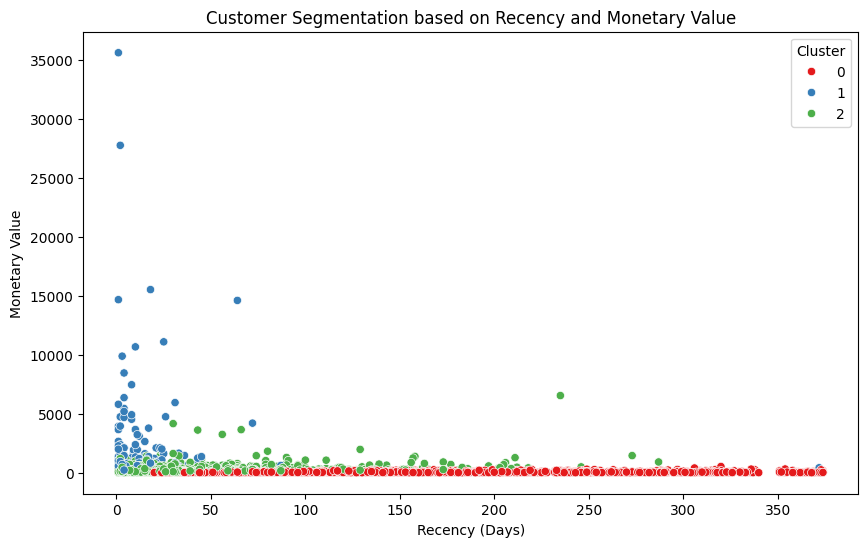
\includegraphics[width=0.7\textwidth]{customer_segments.png}
\caption{Customer segmentation based on Recency and Monetary value.}
\label{fig:segments}
\end{figure}

\subsection{Predictive Modeling}
We implemented Logistic Regression and Random Forest models to predict customer engagement with different campaign types (Email, Social Media, Paid Ads). Table \ref{tab:model_comparison} compares the performance of the two models.

\begin{table}[H]
\centering
\begin{tabular}{|c|c|c|}
\hline
\textbf{Metric} & \textbf{Logistic Regression} & \textbf{Random Forest} \\ \hline
Accuracy        & 0.70                         & 0.66                   \\ \hline
Precision       & 0.00                         & 0.33                   \\ \hline
Recall          & 0.00                         & 0.16                   \\ \hline
F1-Score        & 0.00                         & 0.21                   \\ \hline
\end{tabular}
\caption{Comparison of Logistic Regression and Random Forest models.}
\label{tab:model_comparison}
\end{table}

\section{Discussion}
The findings from this analysis provide key insights for optimizing e-commerce marketing campaigns:
\begin{itemize}
    \item \textbf{Targeting Loyal Customers:} Loyal customers should be rewarded with loyalty programs, exclusive offers, and early access to products to maintain their engagement.
    \item \textbf{Re-engaging At-Risk Customers:} Personalized win-back campaigns, offering discounts or promotions, can help re-engage at-risk customers.
    \item \textbf{Channel Optimization:} Feature importance analysis from the Random Forest model indicated that email campaigns are the most effective, followed by social media and paid ads. Therefore, future campaigns should focus more resources on these channels.
\end{itemize}

\subsection{Limitations and Future Work}
This analysis is based on a sample of the dataset, which may limit its generalizability to the full dataset. Additionally, the simulated campaign data for predictive modeling may not fully reflect real-world customer behavior. Future work could involve incorporating external data sources such as web traffic analytics and demographic data to improve the accuracy of the models.

\section{Conclusion}
This paper applied the SEMMA methodology to analyze customer behavior in the UCI Online Retail dataset. By identifying key customer segments and predicting marketing campaign engagement, we have provided actionable recommendations for optimizing future marketing efforts. The integration of clustering and predictive models has shown that data-driven strategies can significantly enhance customer engagement and ROI in e-commerce marketing.

\begin{thebibliography}{9}
\bibitem{uci_dataset}
UCI Machine Learning Repository. (2012). Online Retail Data Set. \\
\url{https://archive.ics.uci.edu/ml/datasets/Online+Retail}

\end{thebibliography}

\end{document}
